\section{面向服务的架构}

\subsection{面向服务的架构概述}
面向服务的体系结构(SOA)是一种以业务为中心的IT体系结构方法,它支持将您的业务集成为链接的、可重复的业务任务或服务。SOA可帮助用户构建复合应用程序,复合应用程序是利用来自企业内外多个源的功能来支持水平业务流程的应用程序。

在软件工程中,SOA是一组原则和方法,用于以可互操作服务的形式设计和开发软件。这些服务是定义明确的业务功能,构建为软件组件(离散的代码片段和/或数据结构),可以重用于不同的目的。

\begin{itemize}
    \item SOA是从架构方面,整体支持面向服务泛型的基本概念性架构模型。
    \item SOA是一种业务-IT结合的方法。其中,应用依赖于现有的服务来实现业务过程。
    \item 服务是由服务提供商提供并由服务请求者使用的独立可重用软件组件。
    \item 实现SOA主要包括:
    \vspace{-0.8em}
    \begin{multicols}{2}
        \begin{itemize}
            \item 面向服务的企业
            \item 采用服务开发应用
            \item 采用服务对应用进行封装,以便今后的复用
            \item ……
    \end{itemize}
    \end{multicols}
    \vspace{-1em}
\end{itemize}

\begin{wraptable}{r}{6.5cm}
    \centering
    \vspace{-2.5em}
    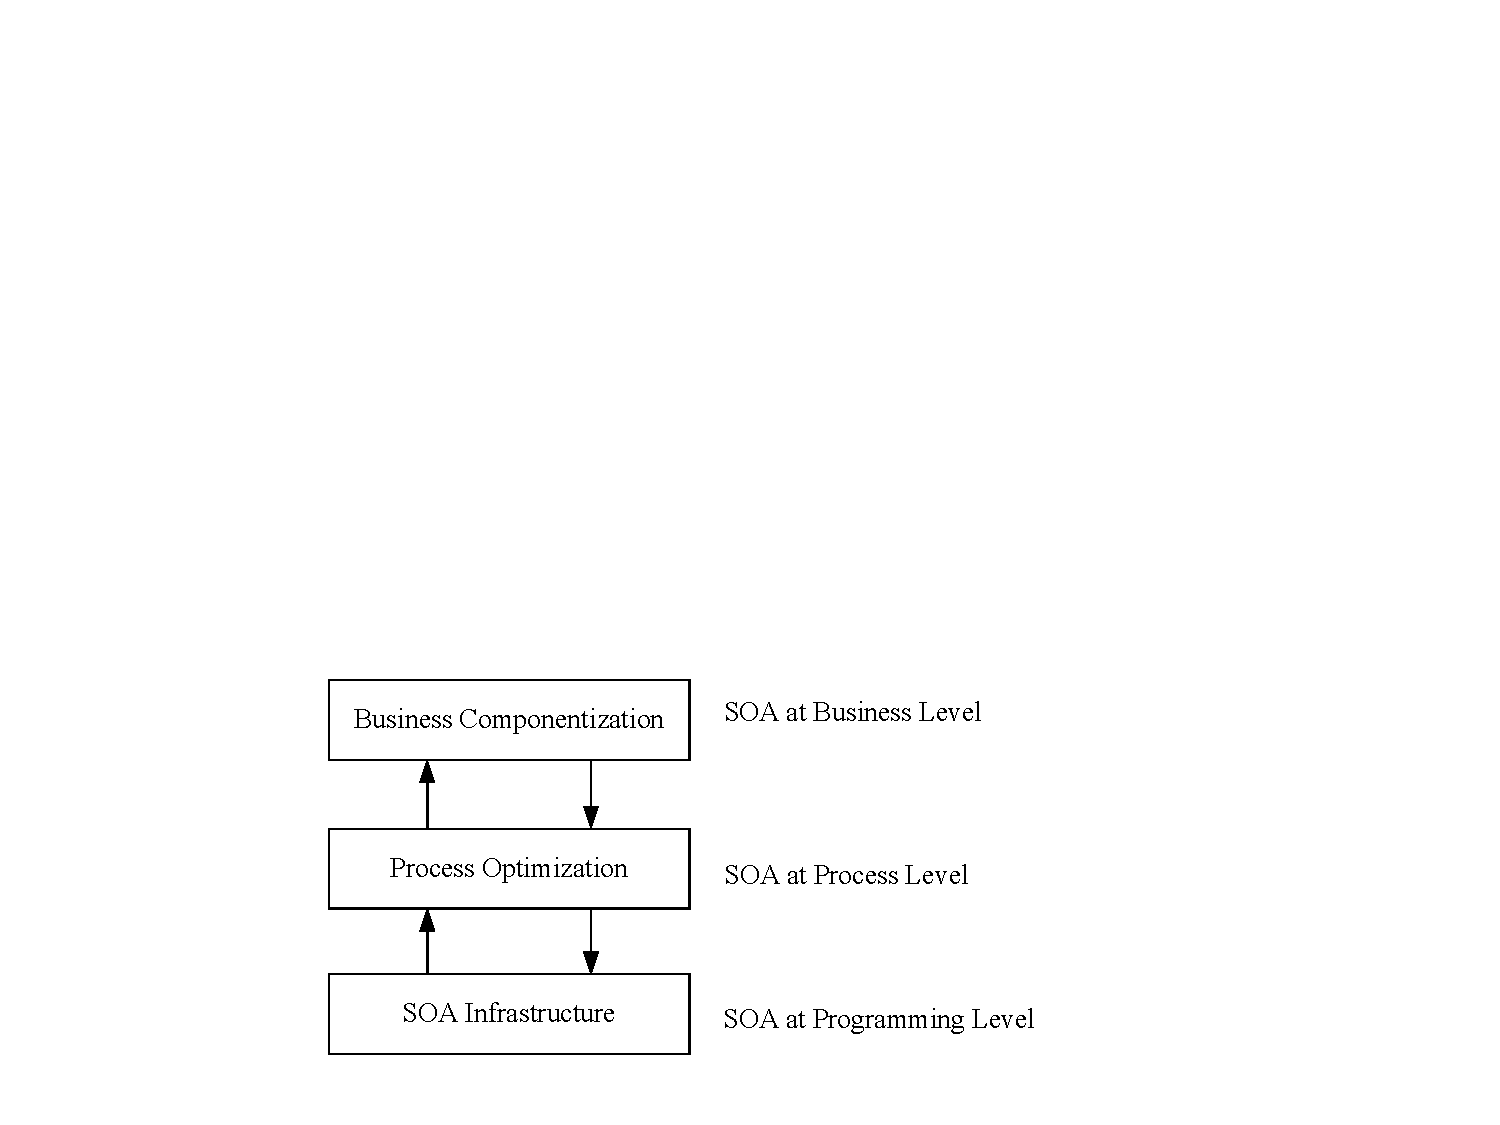
\includegraphics[width=5.5cm]{images/SOA结构.pdf}
    \vspace{-1.5em}
\end{wraptable}
$\ \checkmark\;$SOA解决方案构建在可从Internet或服务注册表访问的可重用服务之上

$\ \checkmark$以标准方式实现复杂软件系统的互操作性和集成

$\ \checkmark$连接IT和业务需求

SOA三角操作模型
\begin{figure}[H]
    \vspace{-0.5em}
	\centering
	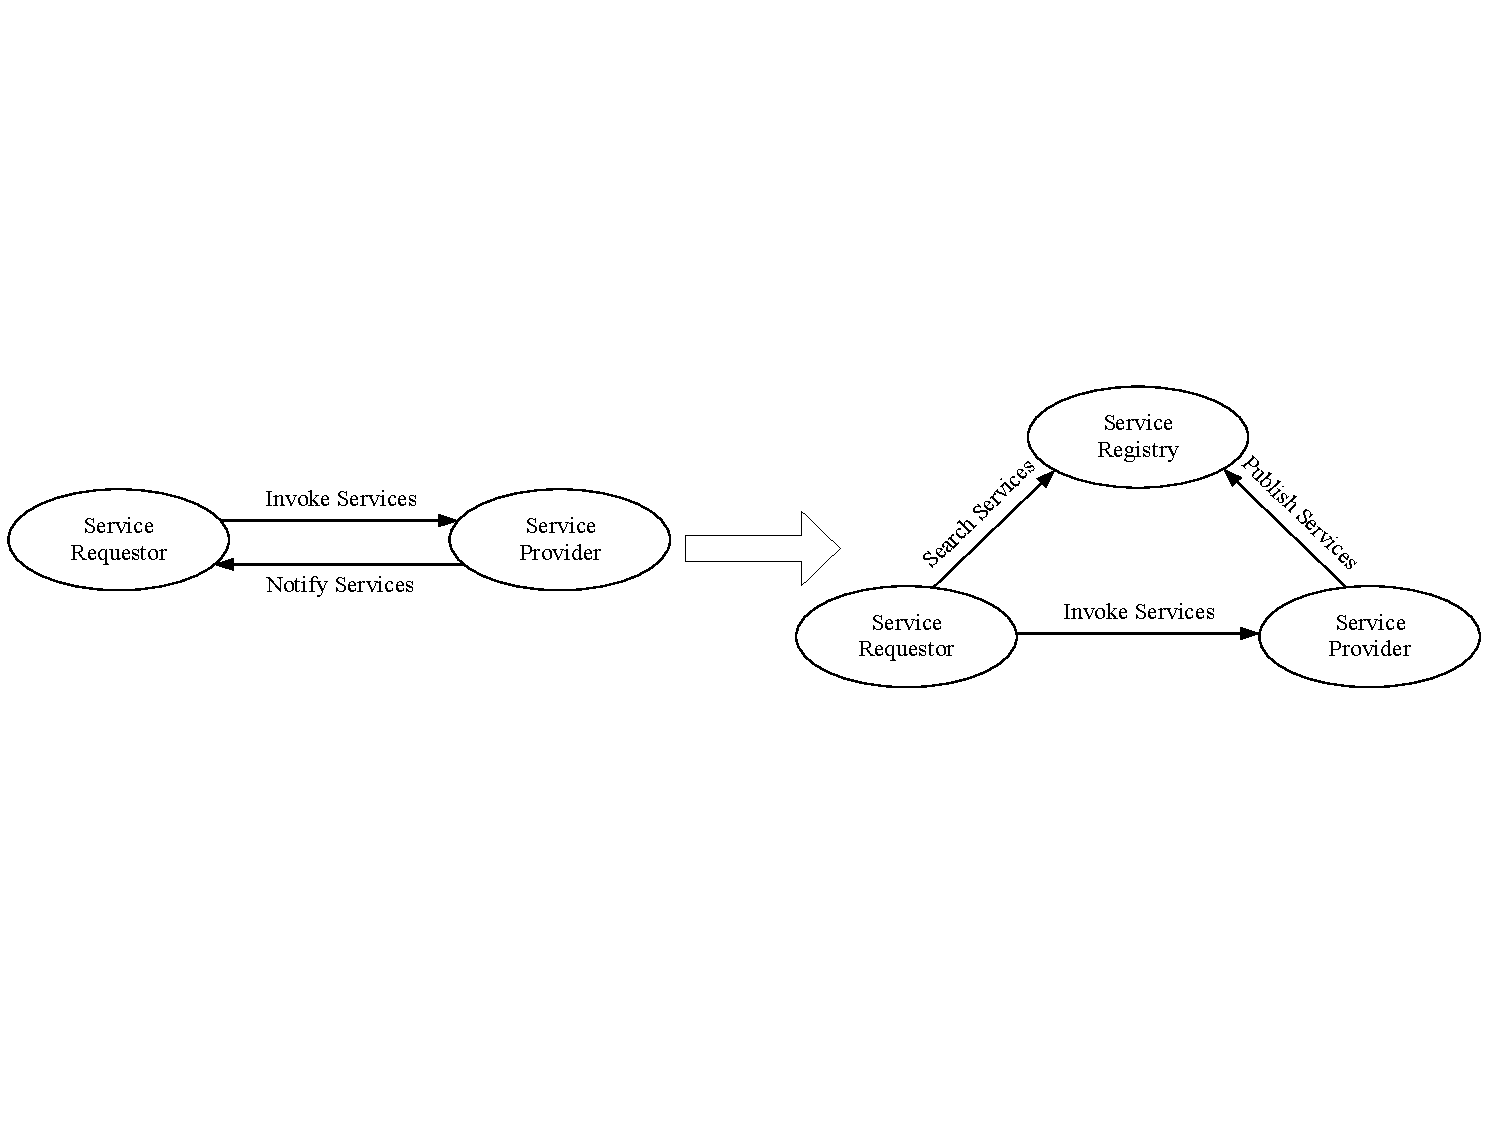
\includegraphics[width=0.85\textwidth]{images/SOA三角操作模型.pdf}
    \vspace{-1em}
\end{figure}

\subsection{SOA的特点}
SOA的优点:
\begin{itemize}
    \item 从IT角度出发
    \begin{itemize}
        \item 松耦合,消除假依赖(复用):语言、平台和厂商中立;消除时间依赖;消除访问地址依赖;消除访问协议依赖
        \item 服务间接寻址(灵活)
    \end{itemize}
    \item 从业务角度出发
    \vspace{-0.8em}
    \begin{multicols}{2}
        \begin{itemize}
            \item 保护企业投资,提升现有IT资源的作用,促进IT资源的复用
            \item 提高企业灵敏度
            \item 支持企业外包管理模式
        \end{itemize}
    \end{multicols}
    \vspace{-1em}
\end{itemize}

从双角度出发,SOA在不同粒度上提供了本质性的指导:业务层、过程层、中间件层和编程层
\begin{itemize}
    \item 在每个层次中间,SOA 按照自顶向下的方式,将一个较大的单元分解为较小、以服务为中心的单元
    \item 按照自底向上的方式,将可供使用的较小单元组织成为较大的单元,用以提供全新的服务
\end{itemize}

\begin{figure}[H]
    \vspace{-0.5em}
	\centering
	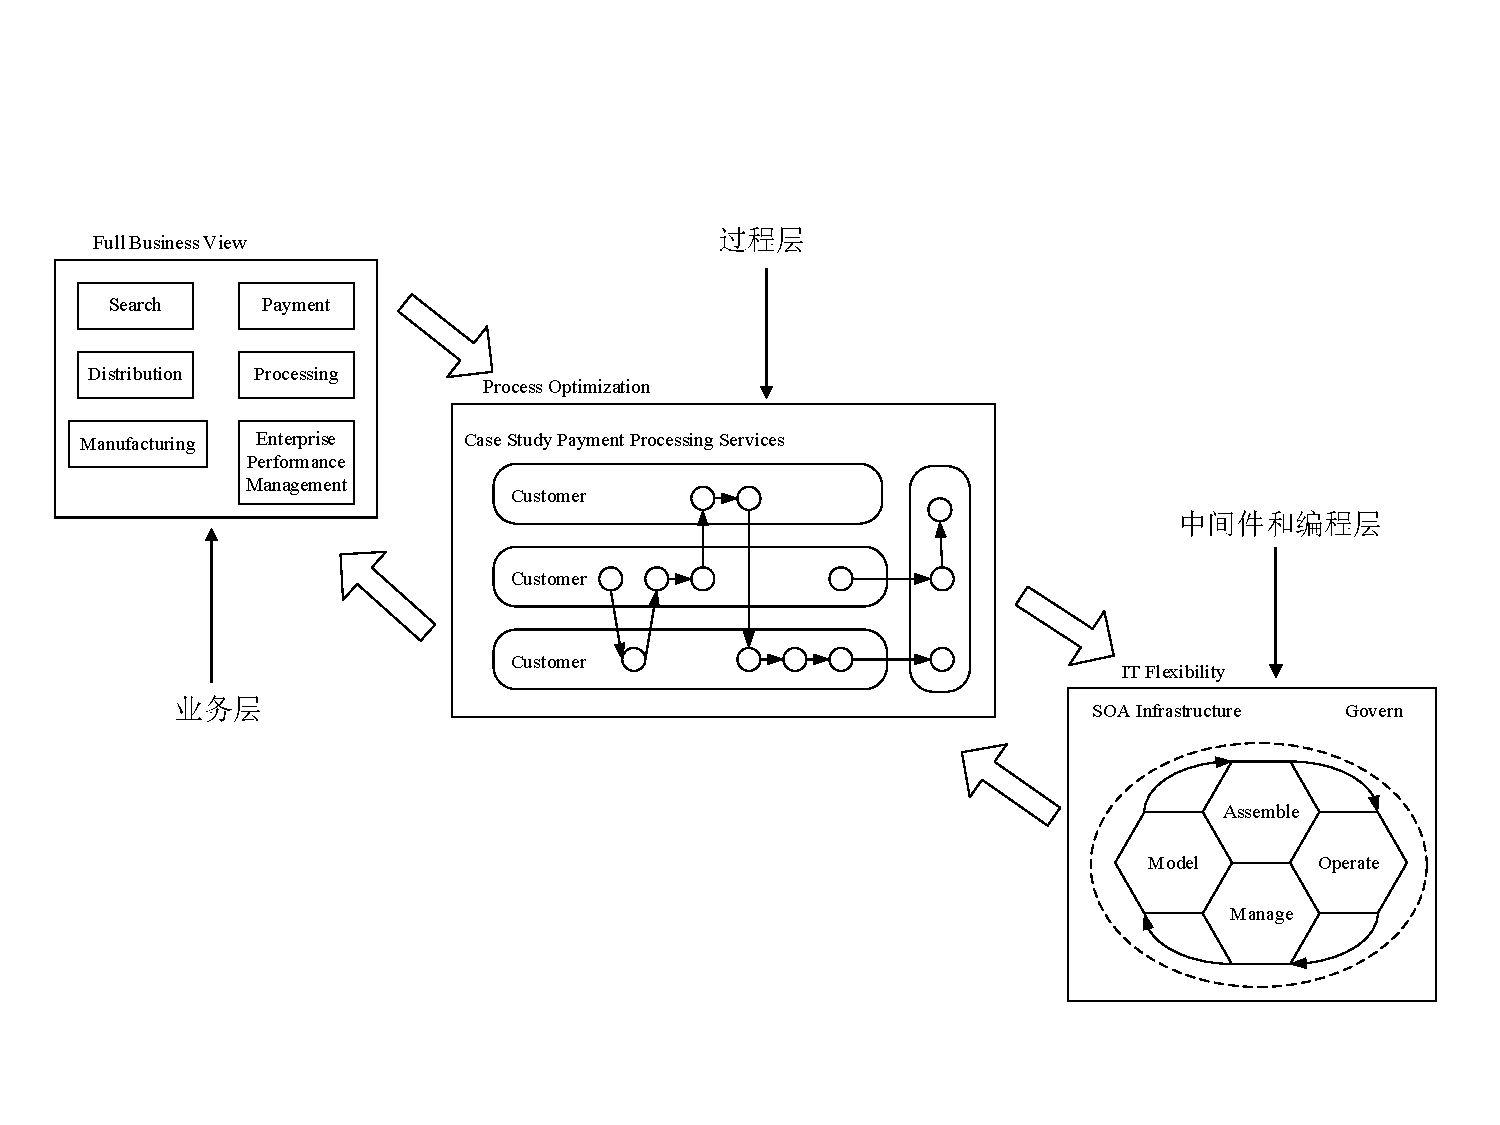
\includegraphics[width=\textwidth]{images/SOA双角度.pdf}
    \vspace{-1em}
\end{figure}

\begin{itemize}
    \item 在编程层,SOA可用于指导低级IT技术
    \begin{itemize}
        \item 简单对象访问协议(Simple Object Access Protocol, SOAP)
        \item 用于数据传输的二进制SOAP消息传递
        \item 服务组件体系结构(Service Component Architecture, SCA,一种编程模型)
    \end{itemize}
    \item 在中间件层,SOA可用于指导通用产品和开源软件的设计和开发
    \begin{itemize}
        \item 从不同的模型中进行选择:例如ESB (Enterprise Service Bus,单个企业服务总线)或多个 ESB、面向消息或基于事件的基础架构
    \end{itemize}
    \item 在过程层,SOA可用于指导业务流程集成和管理,以及事件驱动架构的设计
    \item 在业务层,SOA可用于组件化企业并支持高级转型咨询
    \begin{itemize}
        \item 帮助高管决定是使用SOA服务包实现业务流程,还是使用SOA概念将业务流程划分为子流程
    \end{itemize}
\end{itemize}

\vspace{-0.5em}
\begin{shaded}
\subsubsection*{企业服务总线(ESB)}
\begin{itemize}
    \item ESB是一个概念性的软件基础结构,它促进服务组件及其交互的动态集成、消息路由、中介和控制。
    \item 与通用对象请求代理体系结构(CORBA)对象总线相比,它集成了面向对象的软件组件和Java 2平台企业版(J2EE)应用程序服务器;ESB 在概念上集成了服务和服务组件。
    \item ESB提供了一个基础结构,从集成和消息传递的角度支持服务组件的互操作性和可重用性。
\end{itemize}

ESB的基本形式:
\vspace{-0.8em}
\begin{multicols}{4}
    \begin{itemize}
        \item 集成
        \item 消息路由
        \item 转换
        \item 管理
    \end{itemize}
\end{multicols}
\vspace{-1em}

高级ESB通常提供许多额外的增值功能:
\vspace{-0.8em}
\begin{multicols}{2}
    \begin{itemize}
        \item 用于服务发现和配置的工具
        \item 根据性能和错误事件动态调整服务级别协议
        \item 高级Web服务发现
        \item 适用于现有或新兴技术的特定适配器
    \end{itemize}
\end{multicols}
\vspace{-1em}

\begin{figure}[H]
    \vspace{-0.5em}
	\centering
	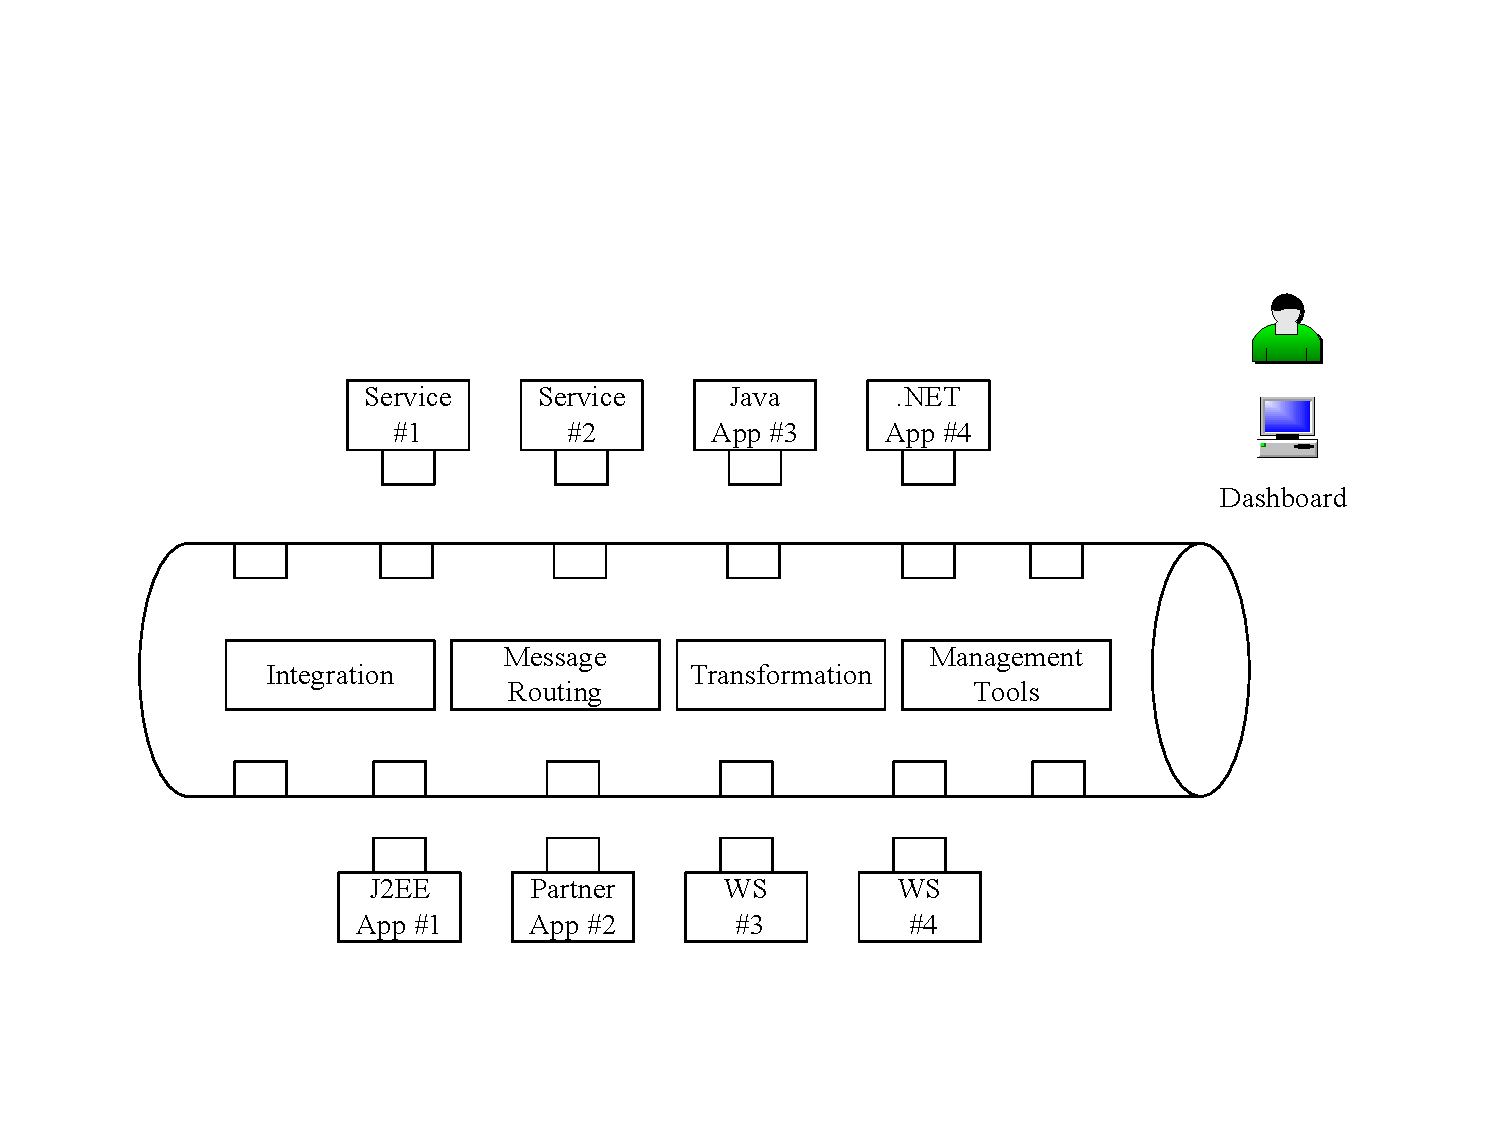
\includegraphics[width=0.65\textwidth]{images/ESB.pdf}
    \vspace{-1em}
\end{figure}

\end{shaded}
\vspace{-1em}

\subsection{SOA参考架构}
\begin{figure}[H]
    \vspace{-0.5em}
	\centering
	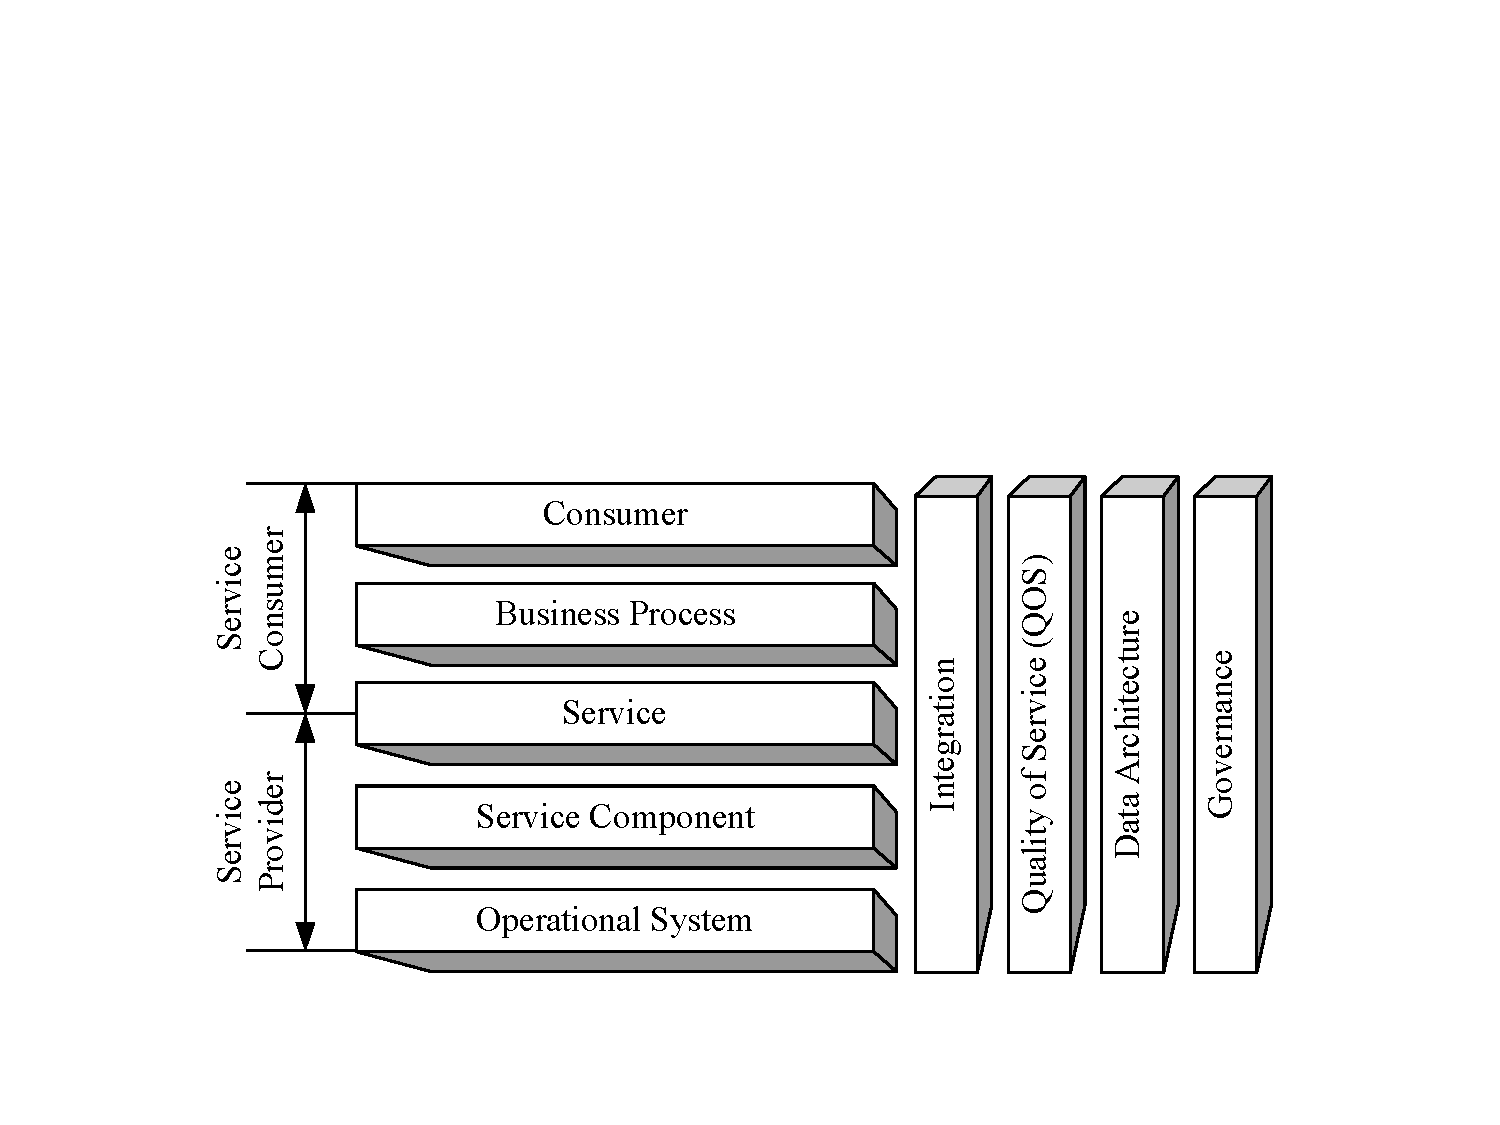
\includegraphics[width=0.7\textwidth]{images/SOA参考架构.pdf}
    \vspace{-1em}
\end{figure}

水平层:对功能性需求加以满足,五个水平层分为服务提供者和服务消费者两组:
\begin{itemize}
    \item 服务提供者(后台)
\end{itemize}
\begin{spacing}{1.2}
    \begin{table}[H]
    \centering
    \vspace{-0.5em}
    \begin{tabular}{|c|l|}
        \hline
        \textbf{操作型系统层} & \begin{tabular}[c]{@{}l@{}}包括ISV(独立软件开发商)提供的打包应用、客户应用、遗留系统等。\\ 该层的应用(不一定面向服务)往往只为一个目的、服务于一类特定用户。\end{tabular}                                                                                                                                         \\ \hline
        \textbf{服务组件层}  & \begin{tabular}[c]{@{}l@{}}包括用于提供用以实现服务层中所定义服务的代码容器,其中一个服务组件依赖于\\ 操作系统型层次中的一些打包组件、服务层中的一些服务、业务过程层中的一些业\\ 务过程。\\ 该层可能实现多个方法,但其中只有一部分会被服务层封装为服务。\\ 从调用角度出发,服务组件层负责完成输入转换和输出配置的自动化逻辑。\end{tabular}                                                       \\ \hline
        \textbf{服务层}    & \begin{tabular}[c]{@{}l@{}}将SOA三角操作模型扩展为综合的逻辑层次,以支持服务注册、服务分解、服务\\ 发现、服务绑定、接口聚合和生命周期管理。服务层负责定位合适的服务提供者,\\ 并绑定到具体目标服务接口;同时负责以服务组合的形式封装服务对外提供。\\ \textbf{服务簇}是服务层中的核心概念,是一类从概念上服务于同一业务功能的服务集合。\\ 服务簇中的服务可以由不同的功能提供者所发布,并在具体的特性上有所差异(但\\ 都能满足业务功能需求)。\end{tabular} \\ \hline
    \end{tabular}
\end{table}
    \vspace{-2.5em}
\end{spacing}

\begin{itemize}
    \item 服务消费者(前台)
\end{itemize}

\begin{spacing}{1.15}
    \begin{table}[H]
    \centering
    \begin{tabular}{|c|l|}
    \hline
    \textbf{服务层}   & 服务层作为前后台连通的接口,功能同上。   \\ \hline
    \textbf{业务过程层} & \begin{tabular}[c]{@{}l@{}}以组合和分解的方式来处理业务逻辑。\\ 从组合角度出发,业务过程层使用服务层来快速组合服务,并协调业务过程来满足消\\ 费者需求;从分解的角度出发,业务过程层将业务需求分解为能够由概念上的服务簇\\ 所表达的任务。\\ 业务服务层着眼于从协作和管理一些列过程的角度出发,采用也无流程来构建SOA\\解决方案。\\ 存在两种组合方式:编排和编导(二者功能上等价,主流模式为编排)。\end{tabular} \\ \hline
    \textbf{消费者层}  & \begin{tabular}[c]{@{}l@{}}消费者层负责表达对业务过程层、服务层及其他层次的调用。\\ 通过为业务服务快速构建用户接口来满足消费者的需求。\\ 消费者层负责构建SOA解决方案与用户之间进行交互的前端接口。\\ 消费者层可能需要同时支持不同种类的用户和渠道。\\ 为了提升展现性能,往往需要支持缓存机制。\end{tabular}                                                         \\ \hline
    \end{tabular}
\end{table}
    \vspace{-1em}
\end{spacing}

\begin{figure}[H]
	\setcounter{subfigure}{0}
	\centering
	\vspace{-0.5em}	
	\subfloat[编排]{
	\begin{minipage}[t]{0.46\linewidth}
	\centering
	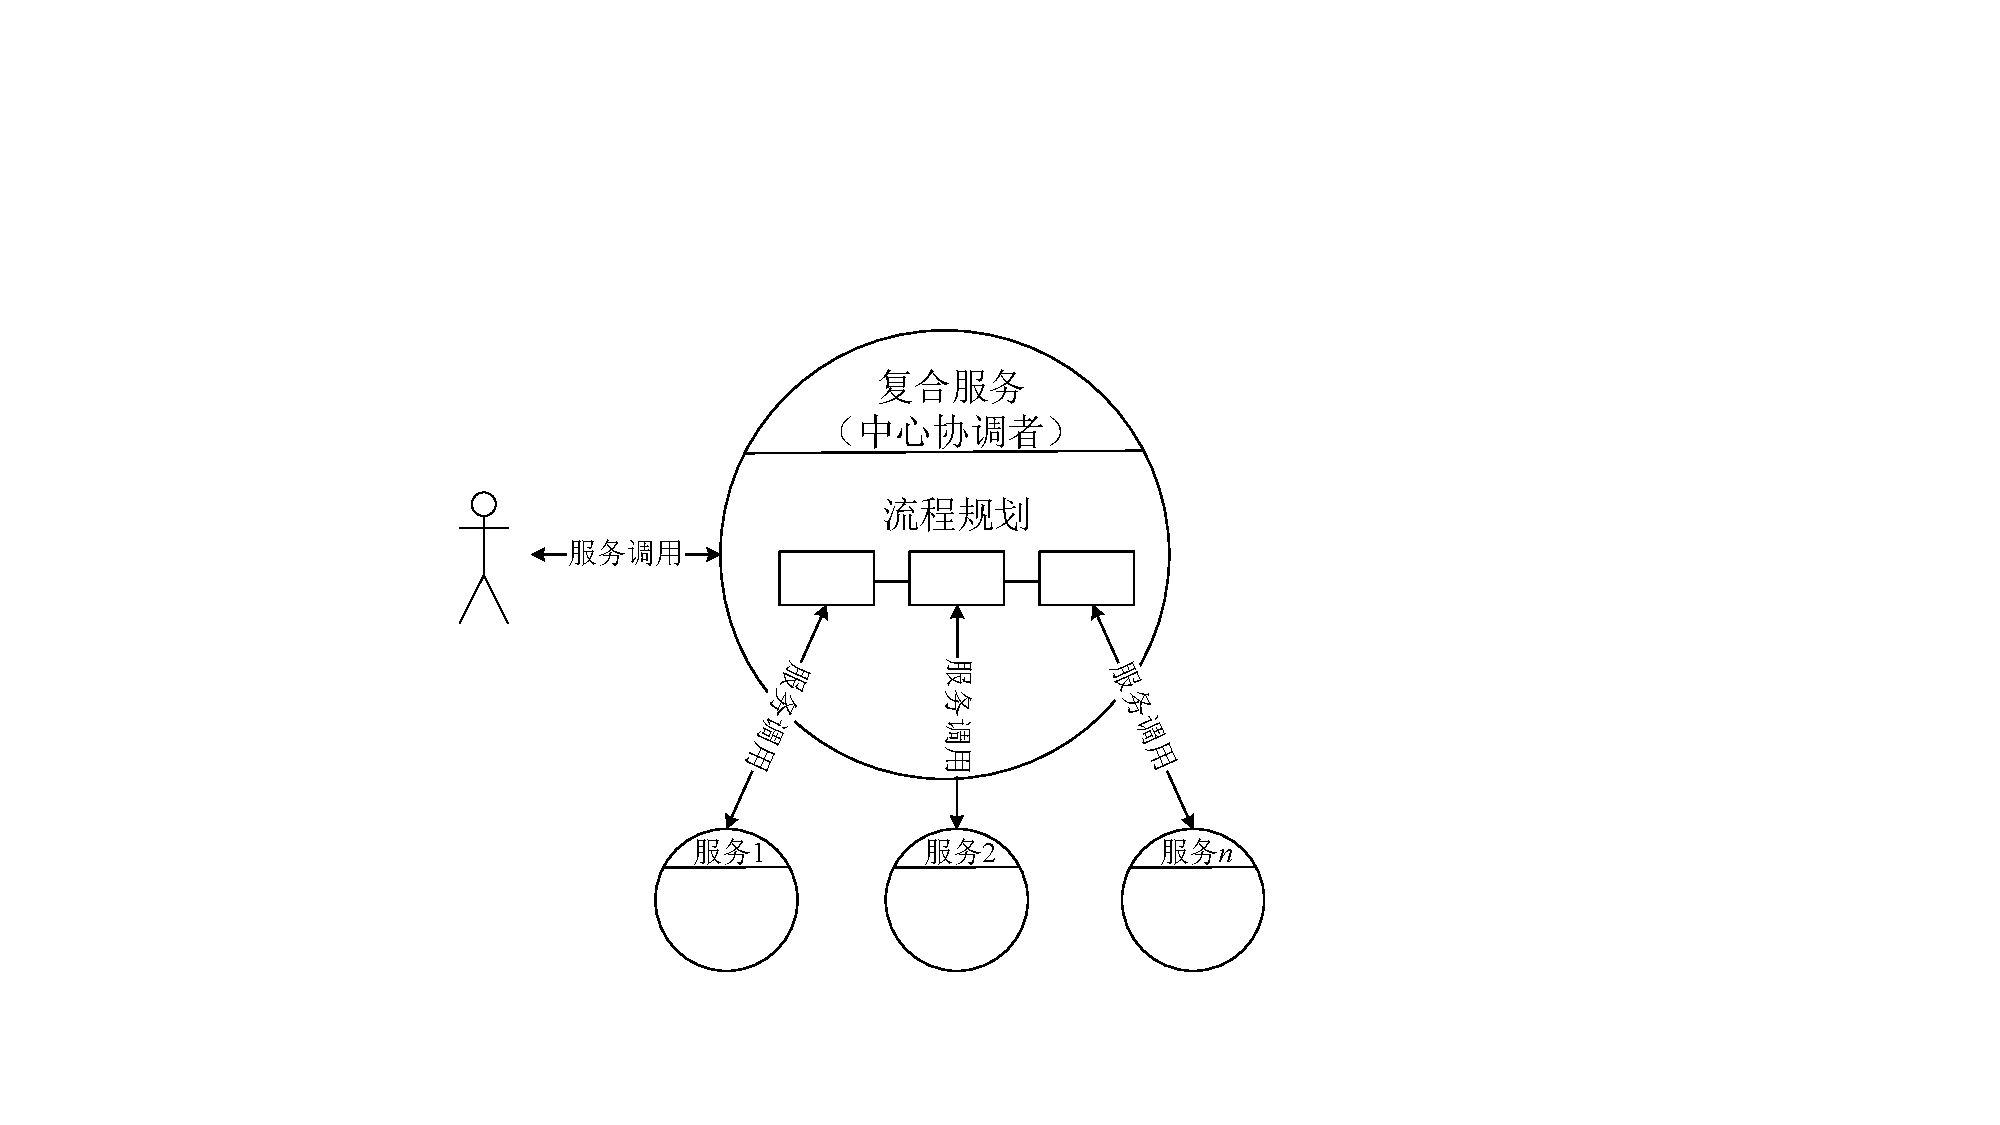
\includegraphics[width=0.97\linewidth]{images/编排.pdf}
	\end{minipage}
	}
    \hfill
	\subfloat[编导]{
	\begin{minipage}[t]{0.47\linewidth}
	\centering
	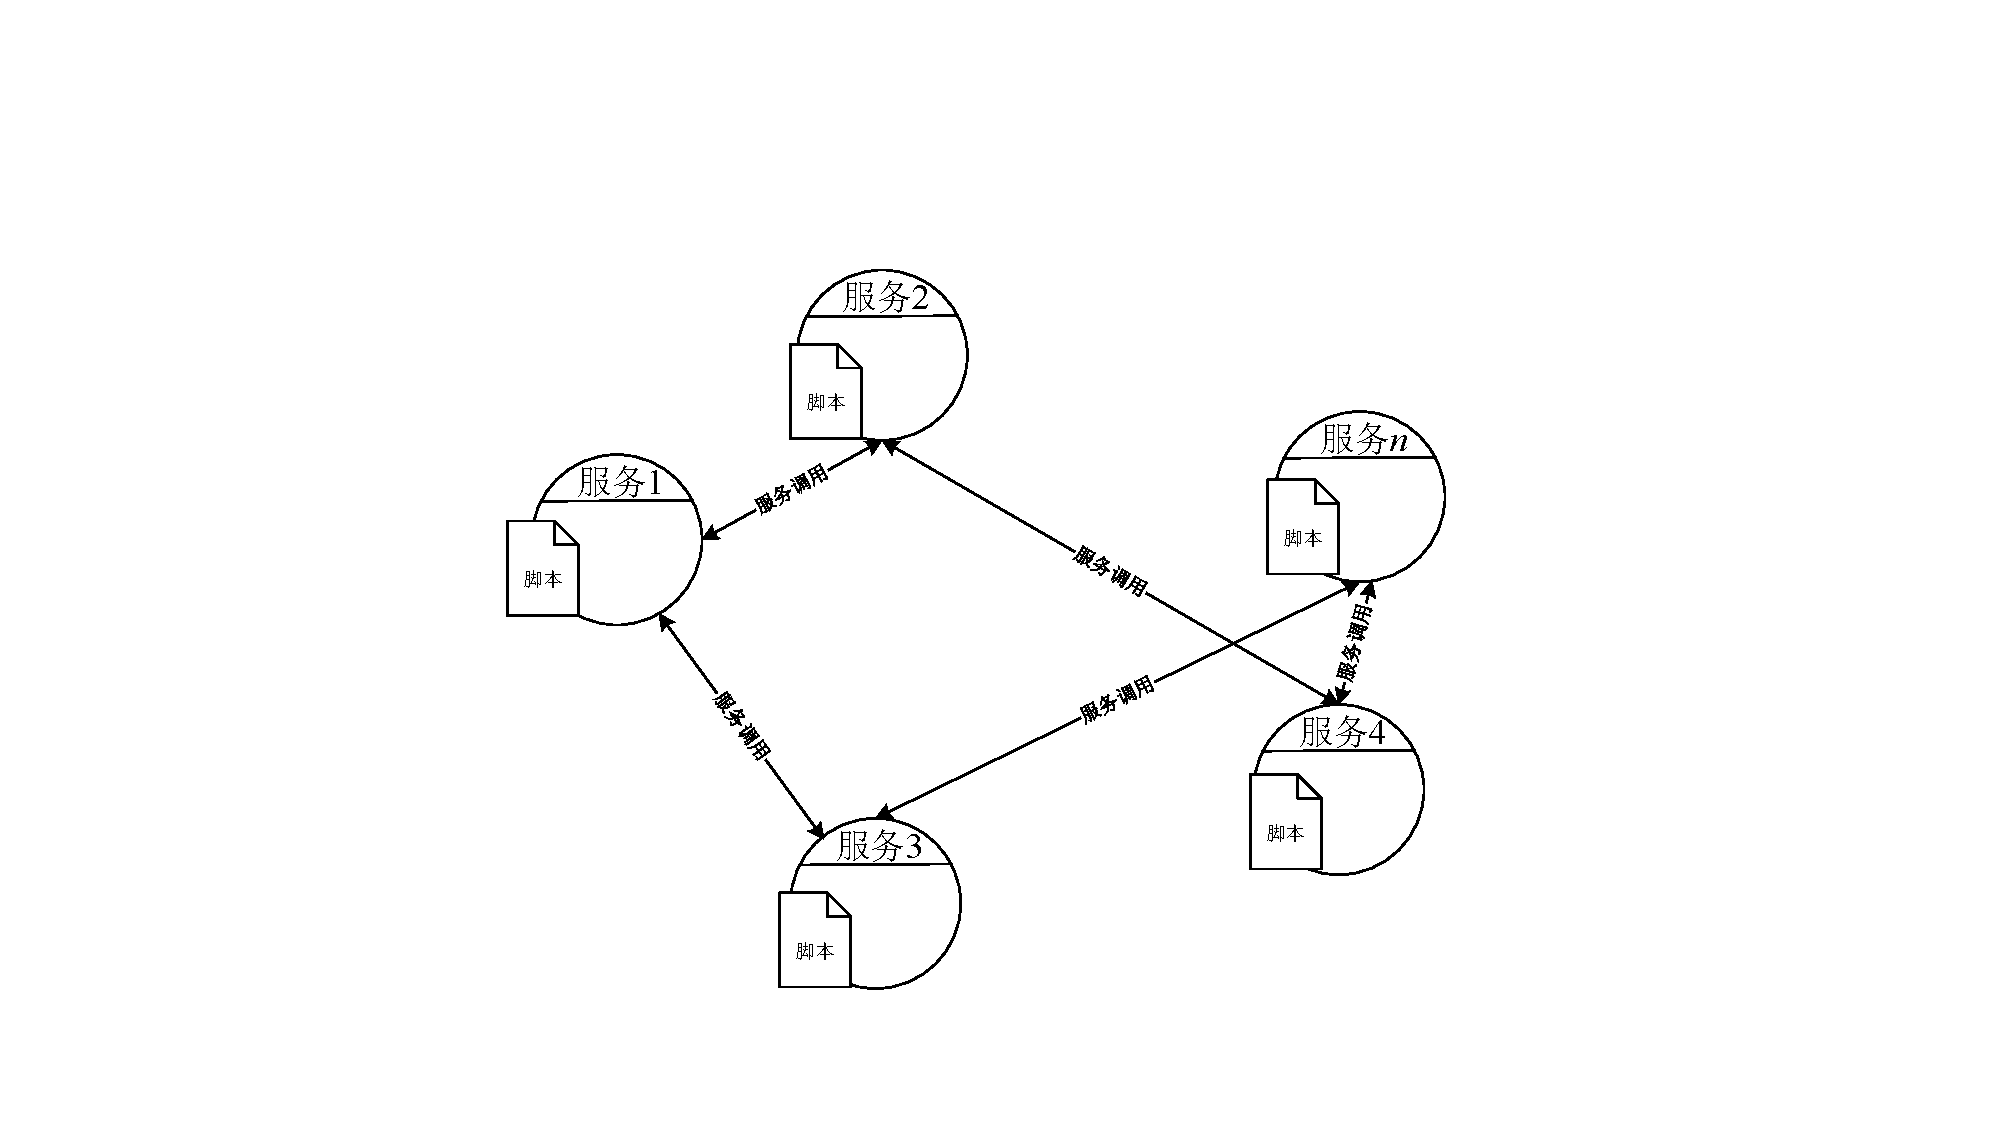
\includegraphics[width=0.97\linewidth]{images/编导.pdf}
	\end{minipage}
	}
	\centering
	\vspace{-1em}
\end{figure}

垂直层:对当前系统进行支撑以及实现服务质量、非功能性需求
\begin{spacing}{1.15}
        \begin{table}[H]
        \centering
        \resizebox{\textwidth}{!}{
        \begin{tabular}{|c|l|}
        \hline
        \textbf{集成层}                                                   & \begin{tabular}[c]{@{}l@{}}SOA解决方案中的关键支持部件,用以在服务请求者和服务提供者之间,完成服务请求的 \\ 中介、路由和转换。\end{tabular}                                                 \\ \hline
        \textbf{\begin{tabular}[c]{@{}c@{}}服务质量层\\ (QoS)\end{tabular}} & \begin{tabular}[c]{@{}l@{}}从各个方面(可用性、可靠性、安全性等非功能性需求)提供解决方案层级的QoS管理。\\ 服务质量层不关注于服务层级的QoS控制,而是着眼于为解决方案层级的 QoS 控制提供 \\ 支持、跟踪、监视和管理。\end{tabular} \\ \hline
        \textbf{数据架构层}                                                 & \begin{tabular}[c]{@{}l@{}}为了方便值链集成(集成来源于不同开发方的服务),数据架构层为领域相关的数据架构提 \\ 供统一的表达和支持机制。\end{tabular}                                             \\ \hline
        \textbf{治理层}                                                   & \begin{tabular}[c]{@{}l@{}}提供用以确保 SOA 解决方案的设计原则;通常使用最佳实践的方式,来提供如何在各个层 \\ 次中构建 SOA 解决方案的原则、如何监管运营中的系统,并在运行时处理异常的原则。\end{tabular}               \\ \hline
        \end{tabular}}
    \end{table}
    \vspace{-2em}
\end{spacing}

\begin{itemize}
    \item SOA-RA 展示了如何将 SOA 解决方案构建为一组逻辑层的抽象。
    \item SOA-RA 是一种松耦合的架构,因为每个层不严格隐藏在上面的层之中。
    \item SOA-RA 是一个企业级架构模板,通过定义参考架构指导在企业级别上创建 SOA 解决方案。
    应用 SOA-RA 模型来定义 SOA 导向的系统架构的一种实践称为服务导向建模和架构(SOMA)。
    \item 在SOA-RA层中配置组件定义了三个步骤:
    \vspace{-0.8em}
    \begin{multicols}{3}
    \begin{itemize}
        \item 服务识别步骤
        \item 服务规范步骤
        \item 服务实现步骤
    \end{itemize}
    \end{multicols}
    \vspace{-1em}
\end{itemize}

\subsection{SOA解决方案生命周期}
服务的生命周期是指从服务开始构思到该服务不再使用时结束的时间段。
\begin{figure}[H]
    \vspace{-0.5em}
	\centering
	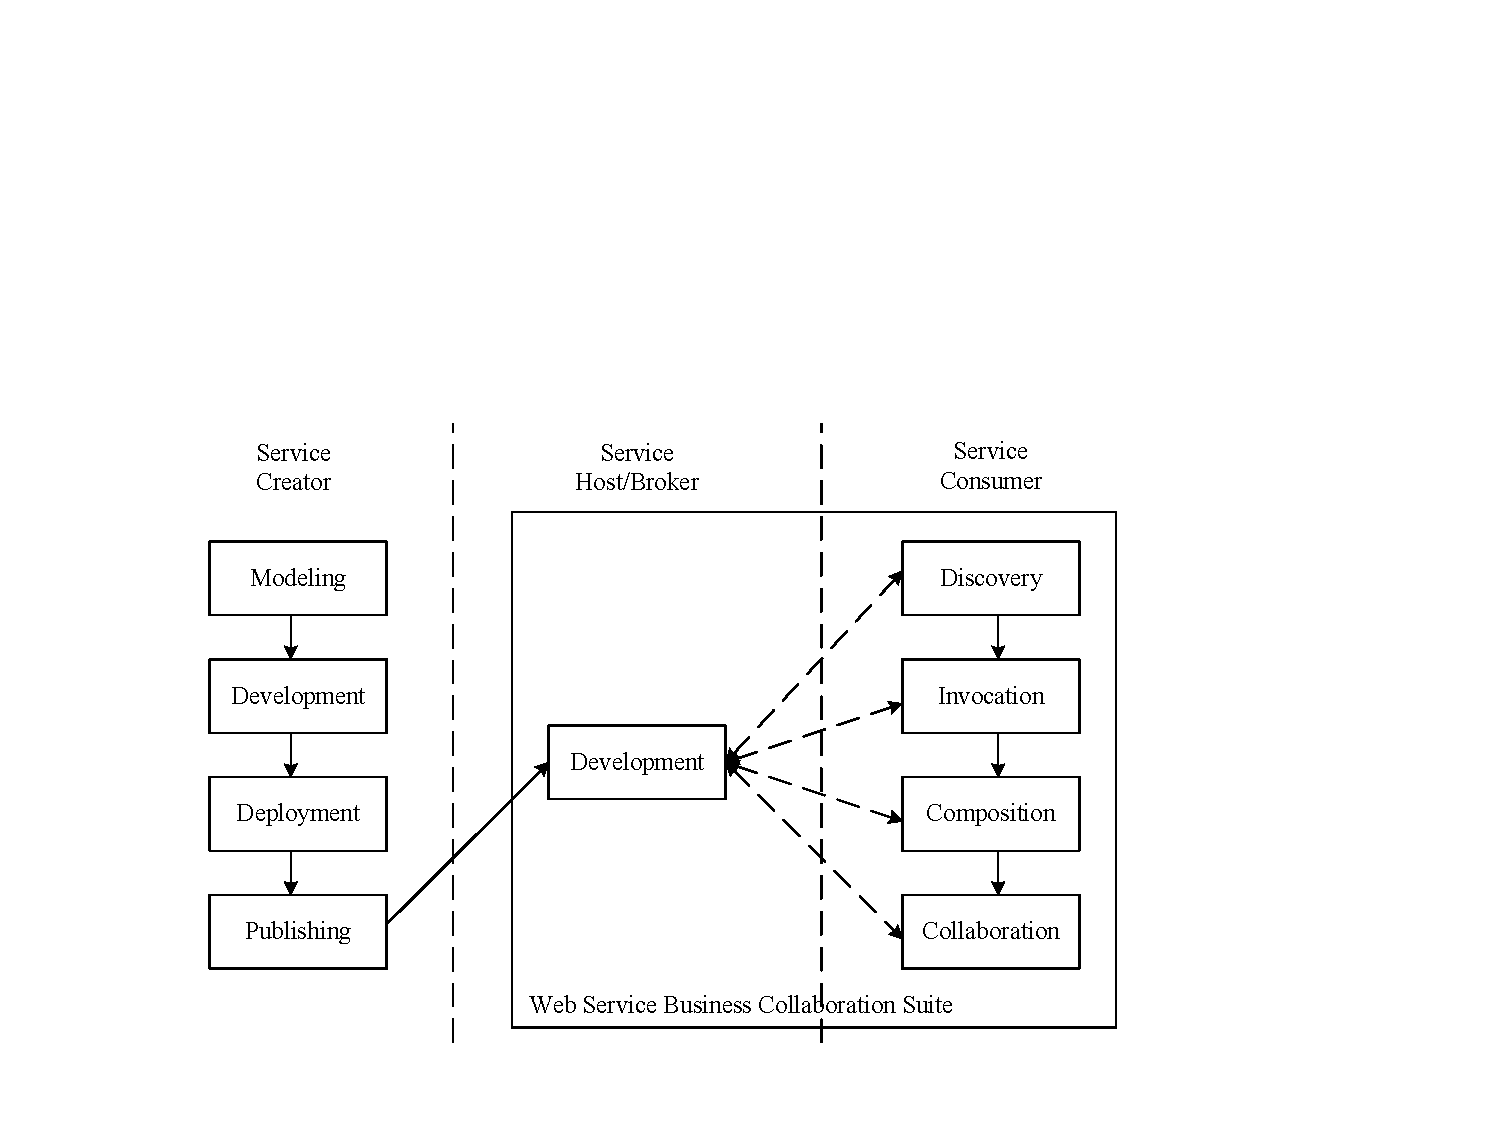
\includegraphics[width=0.65\textwidth]{images/SOA Solution Lifecycle.pdf}
    \vspace{-1em}
\end{figure}

\vspace{-0.5em}
\begin{spacing}{1.2}
\centering
    \begin{longtable}{|m{2.5cm}<{\centering}|m{12cm}|}
    \hline
    服务模型(Services modeling) & 
    \vspace{-1.3em}
    \begin{itemize}[leftmargin=1.5em,itemsep=-2pt]
        \item 使用概念建模技术设计服务
        \item 基于WSDL的自顶向下分解方法是一种服务建模方法
        \item 该方法与传统的接口优先设计方法没有区别
        \item OMG\footnote{OMG(Object Management Group),它是一个国际性的计算机工业标准组织,负责制定和维护各种计算机标准,包括UML和MDA等。该组织致力于推广面向对象技术和相关标准,并促进不同系统之间的互操作性。}的基于UML的模型驱动架构(MDA)可以用于使用Web服务和SOA建模业务解决方案的复杂性
    \vspace{-1.5em}
    \end{itemize} \\ \hline
    开发(Development) & 
    \vspace{-1.3em}
    \begin{itemize}[leftmargin=1.5em,itemsep=-2pt]
        \item 服务的详细实现可以使用任何编程语言来实现(例如Java、C\#和C++)
        \item 服务的开发阶段涉及典型软件生命周期的几个阶段,包括设计、开发和测试
        \item 软件开发方法论可以用于指导开发过程
    \vspace{-1.5em}
    \end{itemize} \\ \hline
    Deployment & \multicolumn{1}{c|}{部署}  \\ \hline
    Publishing & \multicolumn{1}{c|}{发布}  \\ \hline
    Discovery & \multicolumn{1}{c|}{发现服务}  \\ \hline
    调用(Invocation) & 
    \vspace{-1.3em}
    \begin{itemize}[leftmargin=1.5em,itemsep=-2pt]
        \item 通常情况下,服务请求者和服务提供者会就服务级别协议(SLA)进行协商
        \item 在达成共识之后,服务请求者调用所需的Web服务,并在服务提供者现场远程执行服务
        \item SOAP是承载请求和响应的典型协议,需要进行信息的编组和解组
    \vspace{-1.5em}
    \end{itemize} \\ \hline
    组合(Composition) & 
    \vspace{-1.3em}
    \begin{itemize}[leftmargin=1.5em,itemsep=-2pt]
        \item 自适应地将一组可用的Web服务组合成业务流程。
        \item BPEL4WS\footnote{Business Process Execution Language for Web Services,即Web服务业务流程执行语言。它是一种基于XML的编程语言,用于描述在Web服务环境中运行的业务流程,可以协调多个Web服务的协作,实现复杂的业务逻辑。}和Web服务编排接口(WSCI)用于描述这种组合。
    \vspace{-1.5em}
    \end{itemize} \\ \hline
    协作(Collaboration) & 在一个全面的业务流程中,通常会有多个服务由不同的服务提供者提供和调用。
    为了协调它们,它们之间的信息交换和协作是必要的。 \\ \hline
    通过分析控制进行监控和管理(Monitoring and Management with analytical control) & 
    \vspace{-1.3em}
    \begin{itemize}[leftmargin=1.5em,itemsep=-2pt]
        \item 在网络环境中,应监控和控制Web服务的执行
        \item 包括访问控制、性能监控、服务级别协议(SLA)执行和异常处理
        \item 我们应该在涉及多个方的分布式环境中监控和跟踪交换信息的状态
        \item 这个过程可能跨越多个组织,因此需要联合访问控制策略
        \item 进行数据分析和信息分析以改进
    \vspace{-1.5em}
    \end{itemize} \\ \hline
\end{longtable}
\end{spacing}

